The implementation of LM includes a compiler and a virtual machine that runs
byte-code. The virtual machine uses 32 registers for
operations and executes procedures to iterate over the database in order to match facts.
The implementation of the original machine is described in ~\cite{cruz-ppdp14}.
Here, we review the most important details of that paper, while focusing on the
changes for efficiently implementing coordination.

\subsection{Compilation}

The compiler translates each rule to a procedure and a list of facts that need
to exist to satisfy the rule. This procedure is executed by the virtual
machine whenever all the facts mentioned in the body exist.
The procedure loops over all possible combinations of the rule, retrieving facts from the
database, performing join operations and then consuming and deriving facts.
The compiler implements join optimizations (to support efficient rule filtering)
and fact updates (to avoid allocations).

\paragraph{Coordination directives}
Coordination directives are compiled in two different ways, depending on whether they
appear in the body or in the head of the rule. Coordination facts in the body
are compiled into special instructions that inspect the state of the virtual
machine. For example, the directive \texttt{node-priority} will inspect the
target node, retrieve the current priority and assign the priority to a
register. Coordination facts in the head of the rule are also implemented as
special instructions of the virtual machine, but they perform some action,
instead of being added to the database as facts.
Semantically, action facts are like any other. However, since they are
immediately used by the machine, there is no need to store them in the
database, therefore avoiding unnecessary allocations and deallocations.

\subsection{Execution}

The virtual machine is implemented in C++11 and uses the threading system from
the standard library to implement multithreading. Each thread is responsible for
executing a subset of \emph{active nodes}. A node is active if it has unexamined
facts. After a node is processed, it becomes inactive until a new fact is
derived for it. When a new fact is derived for an
inactive node, the node is made active and placed on the appropriate queue of
the appropriate thread.  Threads do useful work by processing active nodes from their queues. Whenever a
thread becomes idle, it attempts to steal nodes from a random thread.
If unsuccessful, the thread becomes idle and waits for program
termination while periodically attempting to steal nodes.

\paragraph{Nodes} 
A node is represented as a collection of facts (per predicate) and an indexing structure that
keeps track of the available facts and potential candidate rules. We need
a separate indexing structure per node since rules run local to each node.

Facts need to be stored efficiently because the virtual machine instructions
perform searches on the database by fixing arguments of a predicate to concrete
values. Each predicate is stored using one of the following data structures:

\begin{tightitemize}
\item \emph{Tries} are used exclusively to store persistent facts.
\item \emph{Doubly Linked Lists} are used to store 
  linear facts. We use a double linked list because we need to efficiently add
  and remove facts.
\item \emph{Hash Tables} are used to improve lookup when 
  linked lists are too long and when we need to do searches filtered by
  a fixed argument. The virtual machine decides which arguments are
  best to be indexed and then uses a hash table
  indexed by the appropriate argument.
\end{tightitemize}

In order to facilitate the implementation of coordination, we added a state
variable for each node. The state machine in
Fig.~\ref{fig:node_states} represents the valid state transitions of a node:

\begin{tightdescription}
   \item[working]: the node is executing.
   \item[inactive]: the node is inactive, i.e., it has no new facts and is not in any
   queue for processing.
   \item[queue]: the node is active with new facts and is in some queue waiting
   to be processed.
   \item[stealing]: the node has just been stolen and is in the process of being
   moved to another thread.
   \item[coordinating]: the node is moving from one queue to another queue.
\end{tightdescription}

\begin{topfig}
   \centering
   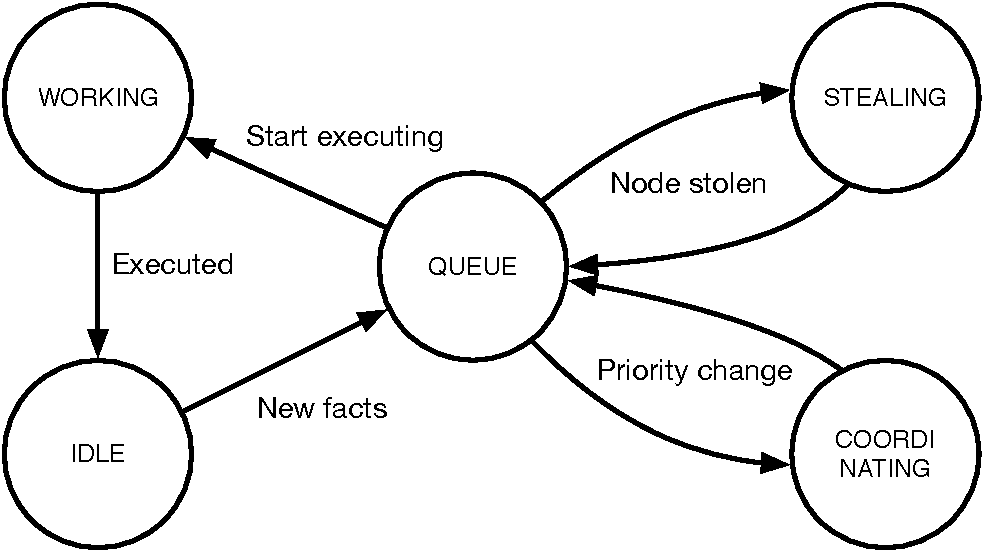
\includegraphics[width=0.3\textwidth]{node_states.pdf}
\vspace*{.5ex}
   \scap{fig:node_states}{The node state machine as represented by the state variable. During
      the lifetime of a program, each node goes through different states as
      specified by the state machine.}
\end{topfig}

Each node is protected by a main spin-lock that allows threads to
change node attributes: incoming facts, owner thread, state variable
and locality information.  A database spin-lock is locked whenever the
node enters into the \textbf{working} state.  

To avoid unnecessary copying, when a node sends facts to a node
located in another thread, the current thread first attempts to lock
the database lock of the target node in order to directly update its
indexing structures, otherwise it adds the facts to the list of
incoming facts that are later processed by the owner thread of the
target node.

\paragraph{Threads}

The main loop for each thread is to get an active node from one of its
local queues and process all applicable rules for that node, generating
new facts, which can result in new facts for the current node or other
nodes.  The thread continues processing facts for the current node
until there are no new facts generated for it.  It will then pick
another active node.  If its queues are all empty it will try to steal
work (i.e., nodes) from another thread.

To support priorities each thread has two pairs of queues: a pair of
doubly linked lists known as the \emph{standard queue} and a pair of
\emph{min/max} heap known as the \emph{priority queue}.  The standard queue
contains nodes without priorities and supports push into tail, remove
node from the head, remove arbitrary node, and remove first half of
nodes.  The priority queue contains nodes with priorities and is
implemented as a binary heap array. It supports the following
operations: push into the heap, remove the \emph{min} node, remove an
arbitrary node, remove half of the nodes (horizontal split), and
priority update.  Operations for removing half of the queue are
implemented in order to support node stealing, while operations to
remove arbitrary nodes or update the priority of nodes allows threads
to change the priority of nodes.

To minimize inter-thread communication, node priorities are
implemented at the thread level. Thus, when a thread picks the highest
priority node from the priority queue, it is only the highest priority
with respect to the set of nodes owned by the thread and not the
highest priority node in the whole program.  

The \texttt{next} and \texttt{prev} pointers of the regular queue are
part of the node structure in order to save space. These pointers are
also used as the index in the priority queue and current priority,
respectively.

Both the regular and priority queue are implemented as a pair of
queues.  This first of the pair is the \emph{static queue} which
contains nodes that cannot be stolen.  The other queue in each pair is
the \emph{dynamic queue} which contains nodes which can be stolen by
other threads.

\paragraph{Communication}

Threads synchronize with each other using mutual exclusion. We use a spin-lock in
each queue to protect queue operations.
Given threads $T_1$ and $T_2$, we enumerate the most important
synchronization intensive places in the virtual machine:

\begin{tightdescription}
   \item[New facts:] When a node executes in $T_1$ and derives facts
   to a node in $T_2$, $T_1$ first buffers the facts 
   and then sends them to the target node. Here, it checks if the
   node is currently \textbf{idle} and then synchronizes with $T_2$ to add the
   node to the $T_2$'s queue.
   \item[Thread activation:] If $T_2$ is inactive when adding facts to a node in
   $T_2$, $T_1$ also synchronizes with $T_2$ to change $T_2$'s state to \emph{active}.
   \item[Node stealing:] $T_1$ synchronizes with $T_2$ when it attempts to steal
   nodes from $T_2$ by removing half of the nodes from one of $T_2$'s queues.
   \item[Coordination:] If $T_1$ needs to perform coordination operations
   to a node in $T_2$, it may need to synchronize with $T_2$ during priority
   updates in order to move the node in $T_2$'s queues.
\end{tightdescription}

\paragraph{Garbage collection}

Whenever a node has an empty database and no references from other nodes, it is
deleted from the graph. The virtual machine uses reference counting to detect
such cases.

\paragraph{Coordination overhead}

In the paper~\cite{cruz-ppdp14}, the LM virtual machine was measured and
compared against implementations of similar programs but written in other
languages. For instance, the Loopy Belief Propagation program was found to be around 2 times slower
than GraphLab, while the N Queens program was found to be around 10 to 15 slower
than a sequential C implementation. Some of those programs were also compared against
a Python implementations and LM faired fairly well. We measured
the impact of the coordination mechanisms implemented for the CLM
virtual machine on regular LM programs and saw very little to no degradation.
Since we also performed general performance improvements, programs such as
PageRank and Greedy Graph Coloring now perform slightly better than before.
